\section{電流パルスを用いたパルス加熱・急冷実験の結果と考察}
本章では電流パルスを用いた半導体スズから金属スズへの変換と共存状態生成に関する実験結果について説明し、筆者の考察を述べる。

\subsection{半導体スズから金属スズへの変換}
本節では電流パルスを用いた半導体スズ(α相)から金属スズ(β相)への変換を行なった実験に関して述べる。

まず1つの薄片(試料6-1)に対してパルス印加の前に抵抗の温度依存性を測定した。図\ref{fig:181213_before_after_pulse_log}に電流パルス前(黒色)の抵抗値を示す。パルス印加前の抵抗は、温度を3K/minで小さくしながら測定したもので、温度が小さくなるほど抵抗が大きくなる半導体的な温度-抵抗依存性を示す。ただし抵抗測定の回路は簡単のため、図\ref{fig:schematics_lockin}の回路からトランス増幅器を取り去ったものとした。
\begin{figure}[!h]
    \begin{center}
   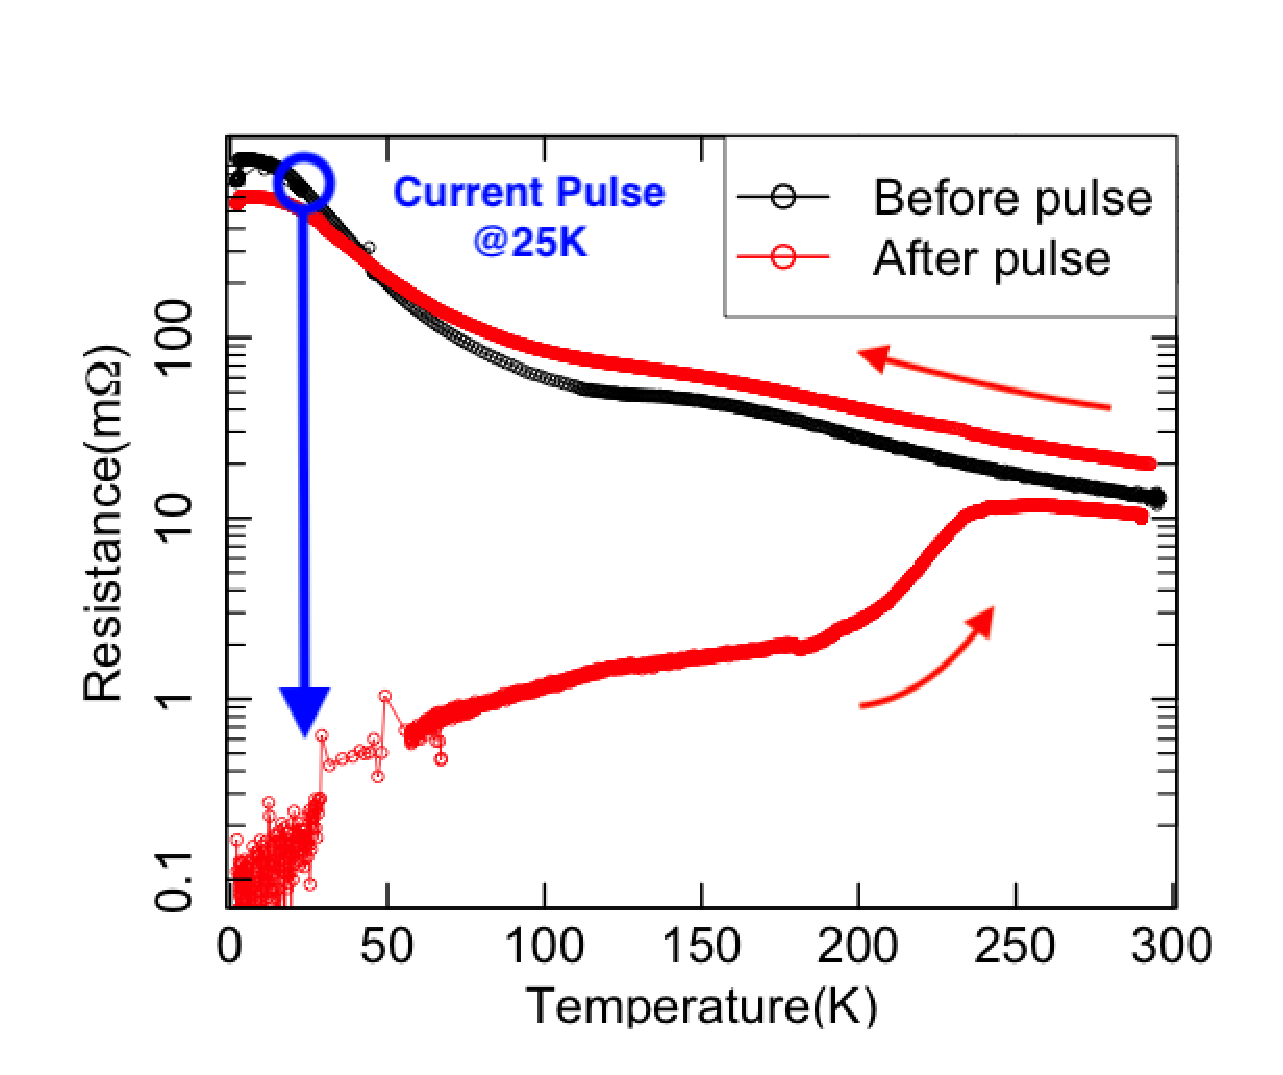
\includegraphics[width=0.7\hsize]{results_discussions/comparison2.eps}
  \end{center}
  \caption{試料6-1の抵抗-温度依存性}
  \label{fig:181213_before_after_pulse_log}
  \end{figure}
 
 %直す
また測定したコンダクタンス(抵抗の逆数)を温度の逆数に対してプロットし、図\ref{fig:181213_before_pulse_Tinv}に示した(アレニウスプロット)。先行研究\cite{Kohnke}によって得られたグラフ(図\ref{fig:conductivity})と同様に0.007 $\rm  K^{-1}$から0.009 $\rm  K^{-1}$(温度110Kから140K)にプラトー領域が現れることが分かる。
\begin{figure}[!h]
    \begin{center}
   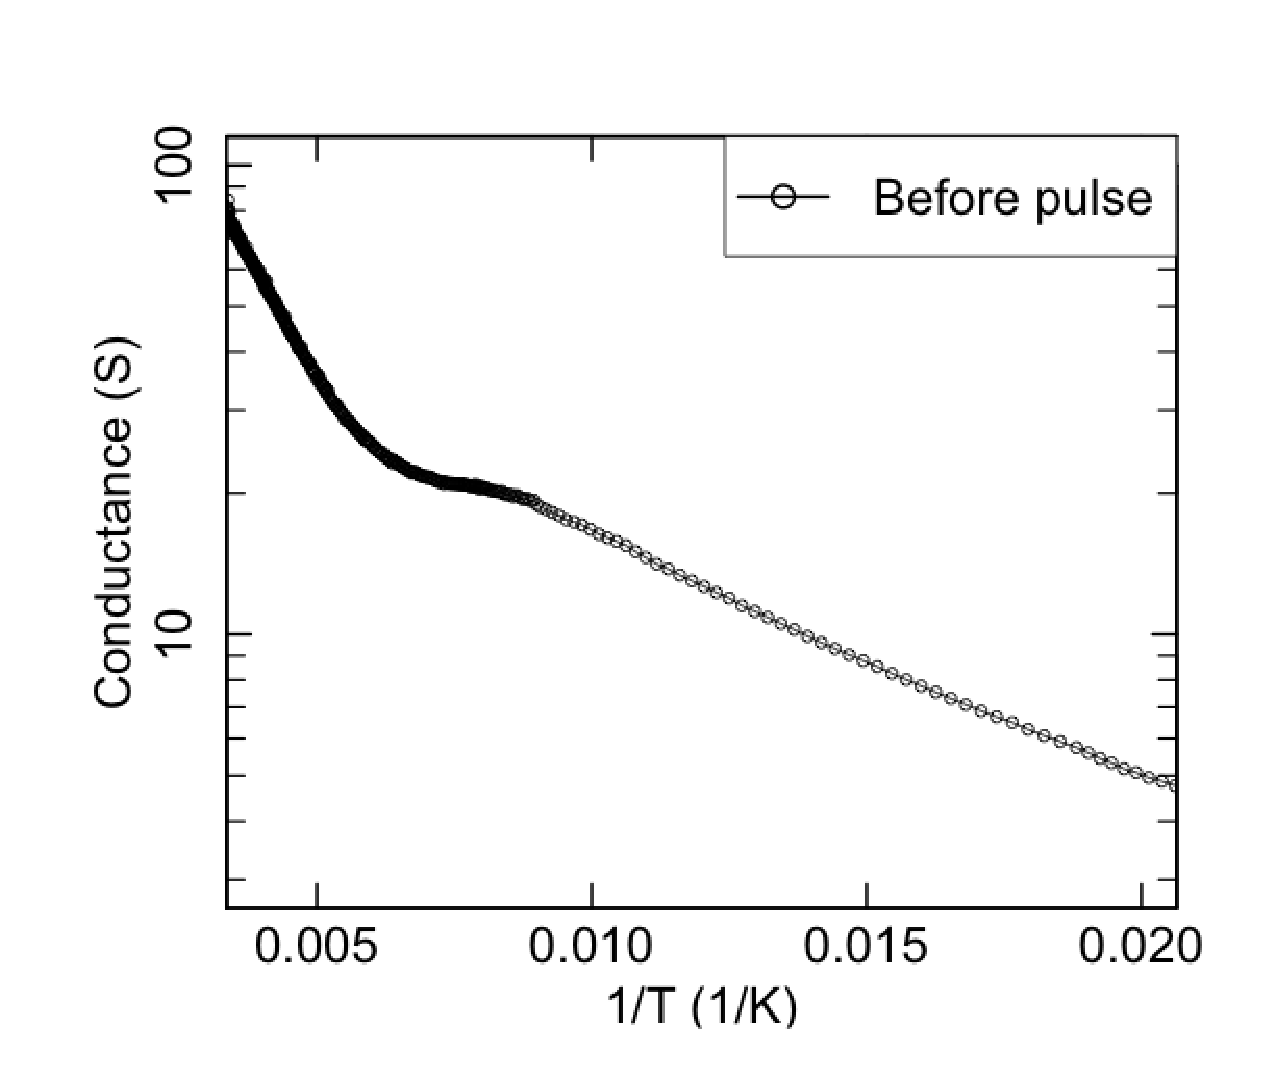
\includegraphics[width=0.6\hsize]{results_discussions/Tinv.eps}
  \end{center}
  \caption{試料6-1の抵抗-温度依存性(アレニウスプロット)}
  \label{fig:181213_before_pulse_Tinv}
  \end{figure}

抵抗の温度依存性を測定した後、次に試料ステージを25Kに保った状態でパルスを印加した。
図\ref{fig:181213_comparison_selected}に、パルス印加時の電流値と抵抗値を示す。3秒間パルス電流を印加した時間は網かけ領域で示した。試料に電流90mA程度の電流パルス(Pulse 1)を印加しはじめてから0.3秒程度の間で抵抗値が半分程度に落ち込み、パルスを切ってから1秒程度で元の値に戻ったことが見て取れる。抵抗の温度依存性の測定(図\ref{fig:181228_before_after_pulse_log})から試料の温度が上がると抵抗が下がることが分かっているので、パルス印加により温度が上昇した。パルス印加中の試料の温度を抵抗からおおまかに見積もると最大40K程度だった。
  \begin{figure}[!h]
    \begin{center}
   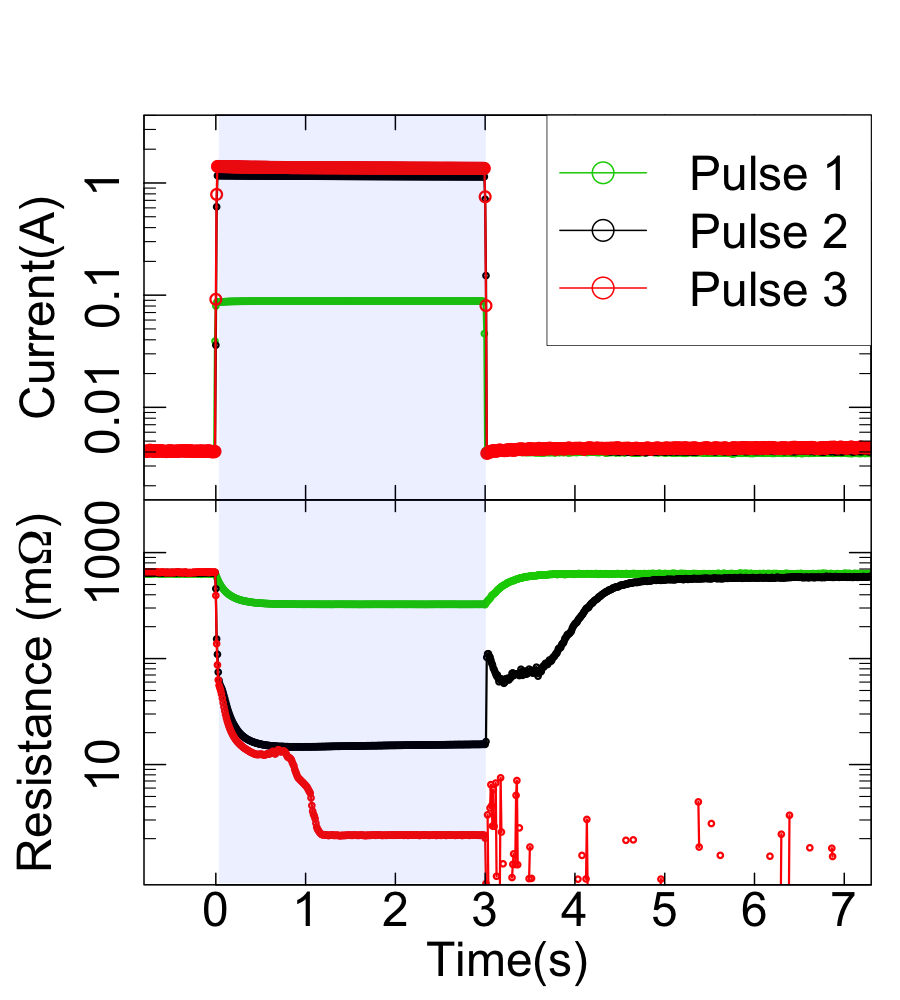
\includegraphics[width=0.6\hsize]{results_discussions/TD2.eps}
  \end{center}
  \caption{試料6-1に流した電流と抵抗の時間変化%\textcolor{red}{電流値の有効数字}
  }
  \label{fig:181213_comparison_selected}
  \end{figure}

電流1140mA程度の電流パルス(Pulse 2)を印加したときも同様に、0.2秒程度で抵抗値が1/10以下に落ち込んだ。抵抗値からパルス中の試料温度を見積もると最大270K程度だった。パルスを切ってから4秒かけると抵抗は元の値の近くに戻ったが、1割程度小さな値となった。

電流1350mA程度のパルス(Pulse 3)を印加したたときも同様に0.2秒程度で抵抗値が1/10以下に落ち込んだが、1秒程度でさらに抵抗値が落ち込み、パルスを切ってからも抵抗は元の値に戻らなかった。パルス前(黒色)とパルス後(赤色)を比較すると、温度25Kで抵抗値は1/1000以下になった。この結果は試料の全体または一部がα$\to$β相転移した可能性を示唆する。

相転移を確認するため、パルス(Pulse 3)後の抵抗値の温度依存性を測定した。抵抗の温度依存性を測定する際は簡単のため図\ref{fig:schematics_lockin}のトランス増幅器を用いなかった。図\ref{fig:181213_before_after_pulse_log}にパルス印加後(赤色)の抵抗温度依存性を示す。パルス印加後(赤色)の抵抗は温度を3K/minで上昇させながら測定したもので、温度を上げると抵抗が大きくなることから半導体的であるよりはむしろ金属的である。

 %直す
図\ref{fig:181213_after_pulse2}にスズの超伝導臨界温度3.7K付近の抵抗を示す。測定時にトランス増幅器を用いなかったため、ノイズが大きいが、スズの超伝導を確認できた。
\begin{figure}[!h]
    \begin{center}
   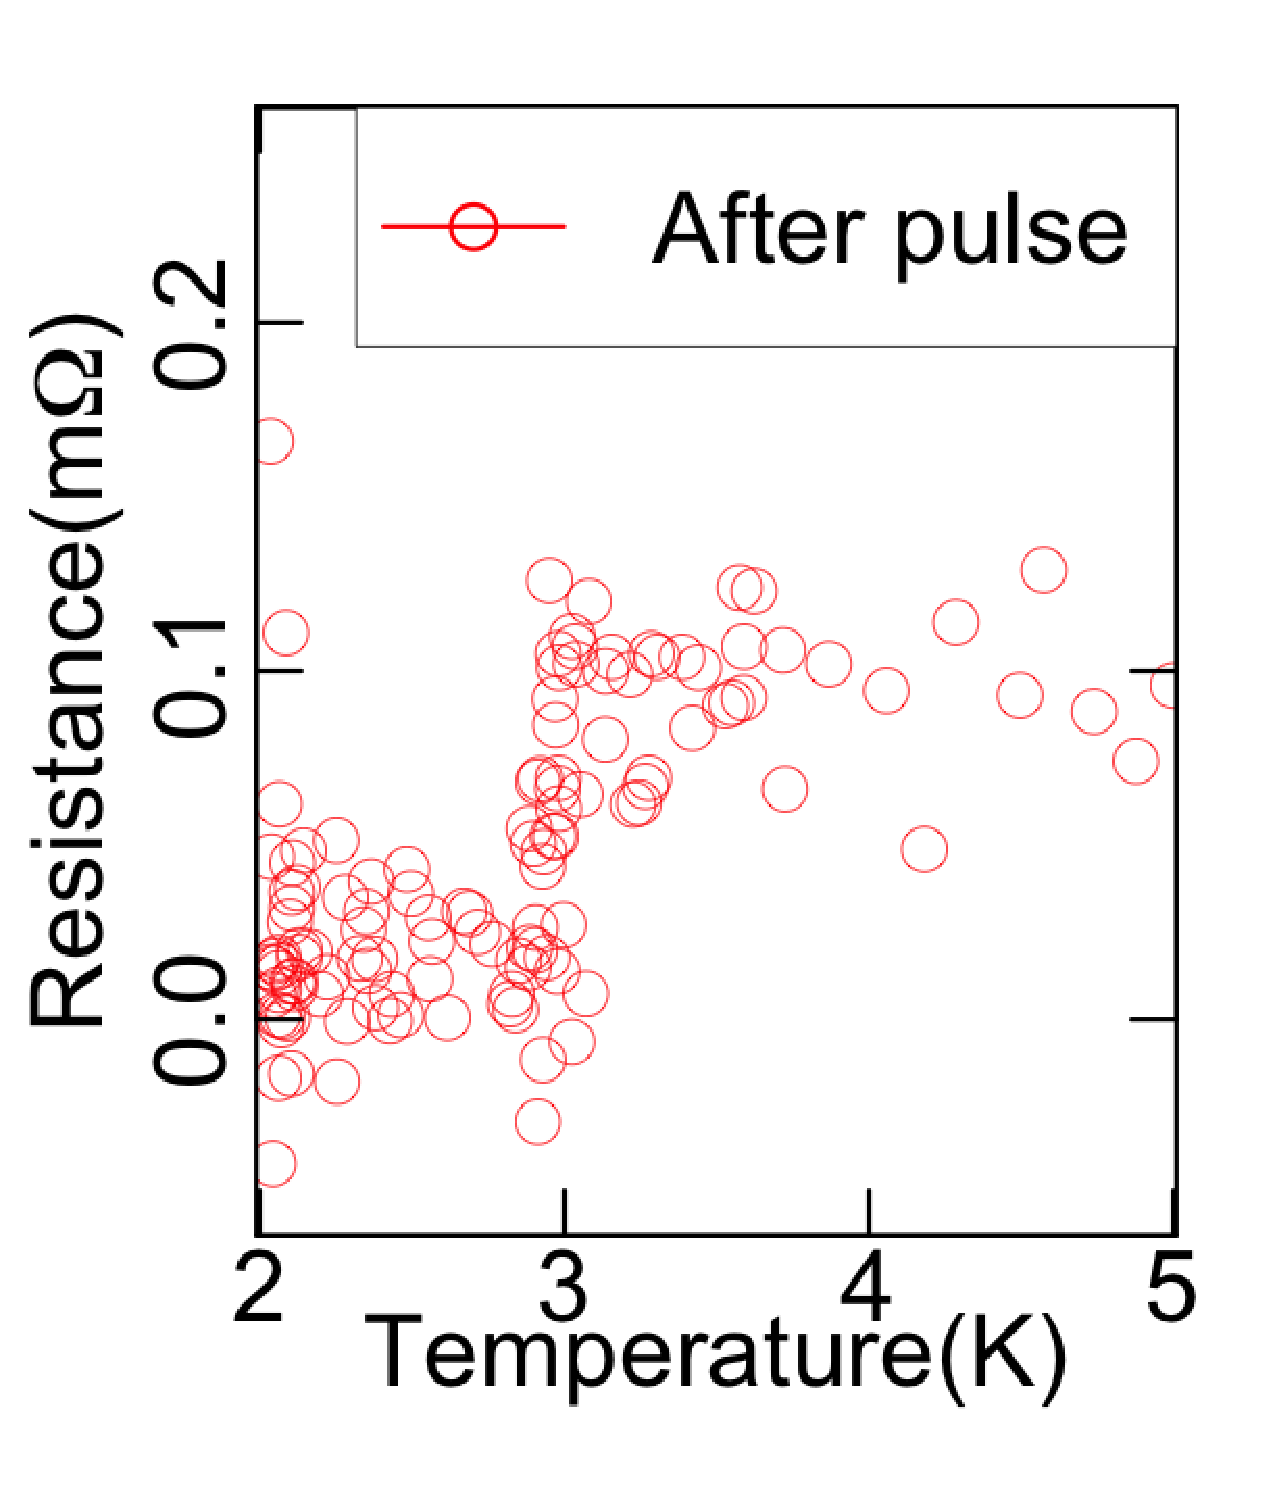
\includegraphics[width=0.4\hsize]{results_discussions/after_pulse2.eps}
  \end{center}
  \caption{試料6-1の低温での抵抗-温度依存性}
  \label{fig:181213_after_pulse2}
  \end{figure}

温度を上げてゆくと200Kから250Kの間で試料の抵抗値が大きく増加し、βスズ(金属)からαスズ(半導体)の抵抗値に戻った。この結果はβ$\to$α相転移が再度起こったことを示唆する。

200Kから250Kの間でβ$\to$α転移が起こったことを確かめるために、再度試料6-1の抵抗の温度依存性を温度を3K/minで下げながら測定し、図\ref{fig:181213_before_after_pulse_log}に示す。ただし測定の際は試料の電圧降下をトランス増幅器で増幅した(図\ref{fig:schematics_lockin})。温度が小さくなるほど抵抗が小さくなる半導体的な温度-抵抗依存性を示すことから、200Kから250Kの間でβ$\to$α転移が再び起こったことが分かる。
\begin{figure}[!h]
    \begin{center}
   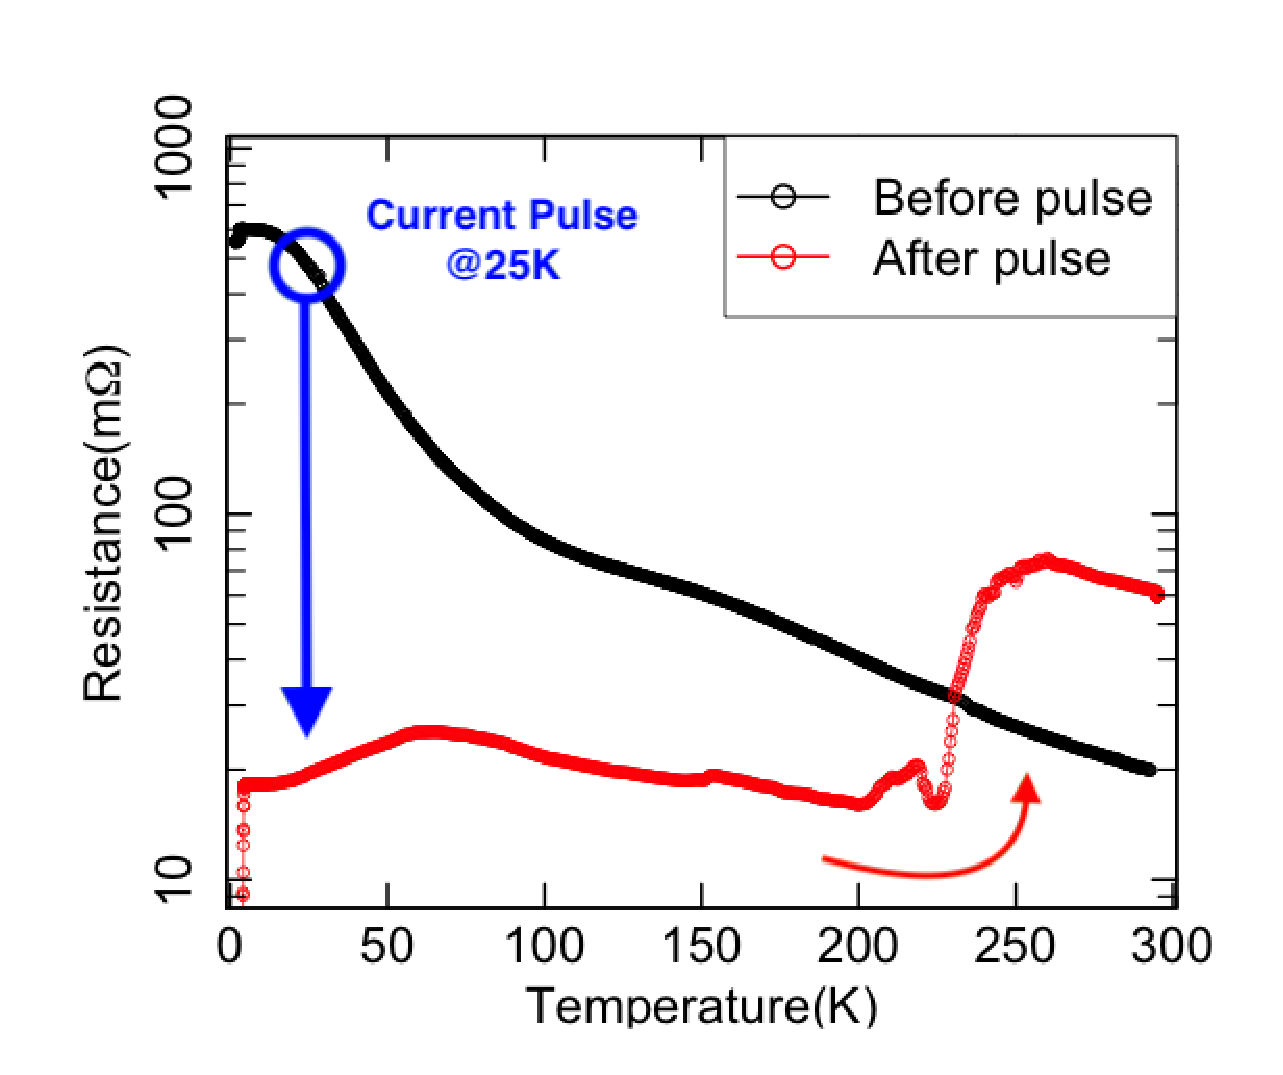
\includegraphics[width=0.7\hsize]{results_discussions/comparison3.eps}
  \end{center}
  \caption{試料6-1の抵抗-温度依存性(2回目)}
  \label{fig:181228_before_after_pulse_log}
\end{figure}

さらにこの試料6-1を25Kに保った状態で再度パルスを印加し、α$\to$β転移の再現性を確認するとともに、繰り返し変換が可能であることを実証した。図\ref{fig:181213_comparison_selected}に、パルス印加時の電流値と抵抗値を示す。3秒間のパルス電流を印加した時間は網かけ領域で示した。
\begin{figure}[!h]
    \begin{center}
   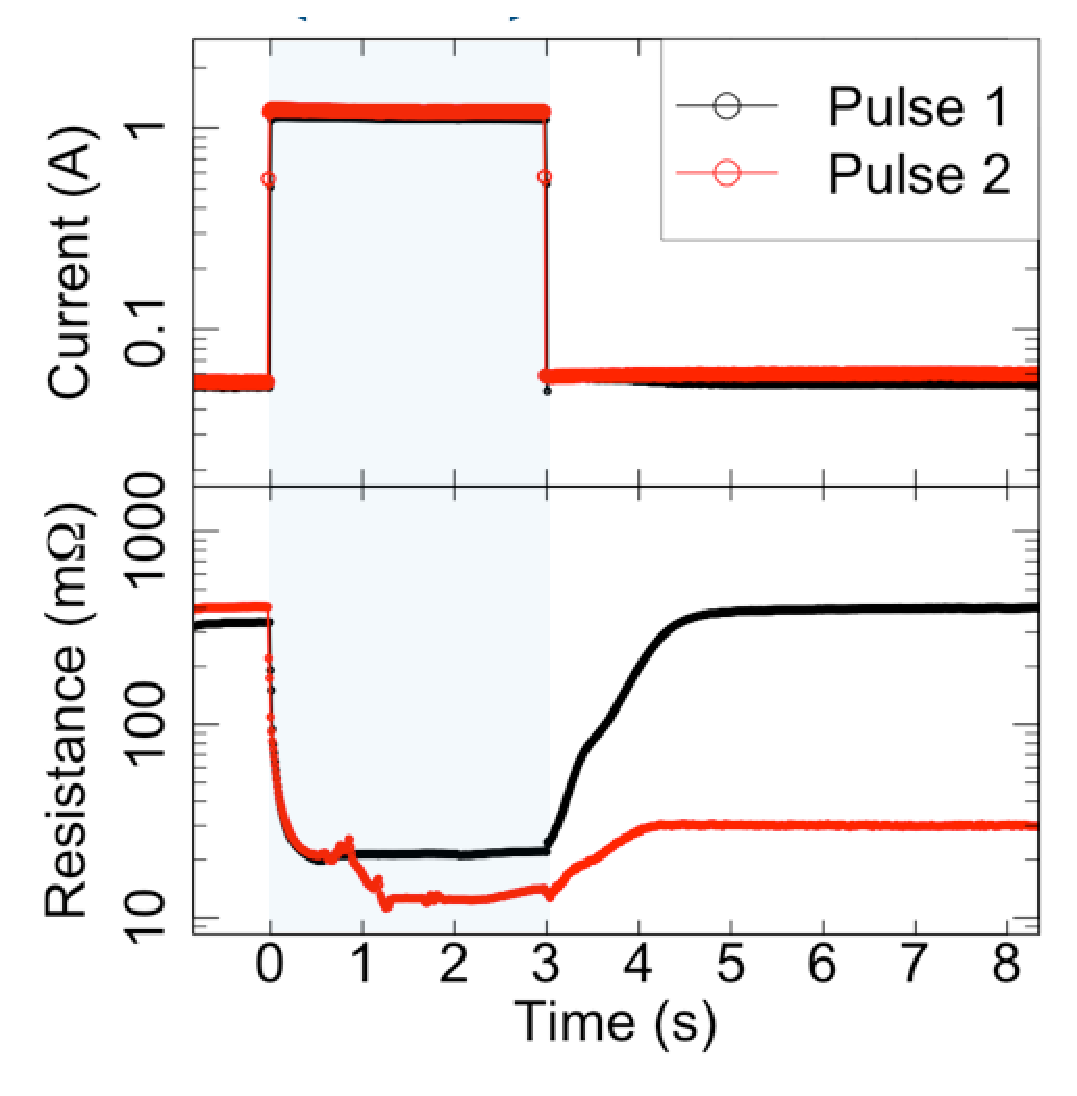
\includegraphics[width=0.6\hsize]{results_discussions/TD1.eps}
  \end{center}
  \caption{試料6-1に流した電流と抵抗の時間変化(2回目)}
  \label{fig:181228_current_resistance.eps}
\end{figure}

電流1100mA程度の電流パルス(Pulse 1)を印加したときは、0.2秒程度で抵抗値が1/10程度に落ち込んだ。抵抗値からパルス中の試料温度を見積もると最大280K程度だった。パルスを切ってから4秒かけると抵抗は元の値の近くに戻ったが、1割程度大きな値となった。電流1200mA程度のパルス(Pulse 2)を印加したたときも同様に0.2秒程度で抵抗値が1/10程度に落ち込んだが、1秒程度でさらに抵抗値が落ち込み、パルスを切ってからも抵抗は元の値の近くに戻らなかった。%しかしわずかに抵抗が上昇したことから、αスズが部分的にβスズに変換された可能性が示唆される。

さらにパルス印加後の抵抗の温度依存性を測定した。図\ref{fig:181228_before_after_pulse_log}(赤色)に示す。パルス印加後の抵抗は67Kに極大を持つ。またパルス前(黒色)とパルス後(赤色)を比較すると、温度25Kで抵抗値は1/20以下になった。前回の抵抗が1/1000となった結果と比較すると、部分的にα$\to$β転移が起きた可能性が示唆される。

実際、部分的にα$\to$β転移が起きて、金属と半導体が並列抵抗のネットワークを作っているとして抵抗値の振る舞いは理解できる。半導体スズ中に部分的にだけ金属スズが現れているとき、試料の抵抗値は半導体スズと金属スズの間となる。これからパルス前後の抵抗値を比較するとパルス後は温度25Kで1/20程度の大きな値になったことが説明できる。また温度が高くなると抵抗が小さくなる半導体の特性と、温度が高くなると抵抗が大きくなる金属の特性から、67Kに抵抗値の極大ができることも理解できる\cite{Mayr,McLachlan}。

図\ref{fig:181228_after_pulse}に温度6K以下におけるパルス前後の抵抗を示す。抵抗測定の際はトランス増幅器を用い、特にパルス後には試料ステージを0.005K/minで加熱しながら抵抗測定した。パルス後の抵抗を温度5Kと3Kで比較すると$10^{-4}$以下に落ち込み、超伝導転移が起こっていることが分かる。臨界温度を見積もると4Kだった。スズの臨界温度3.7Kに近い値である。
\begin{figure}[!h]
\begin{center}
   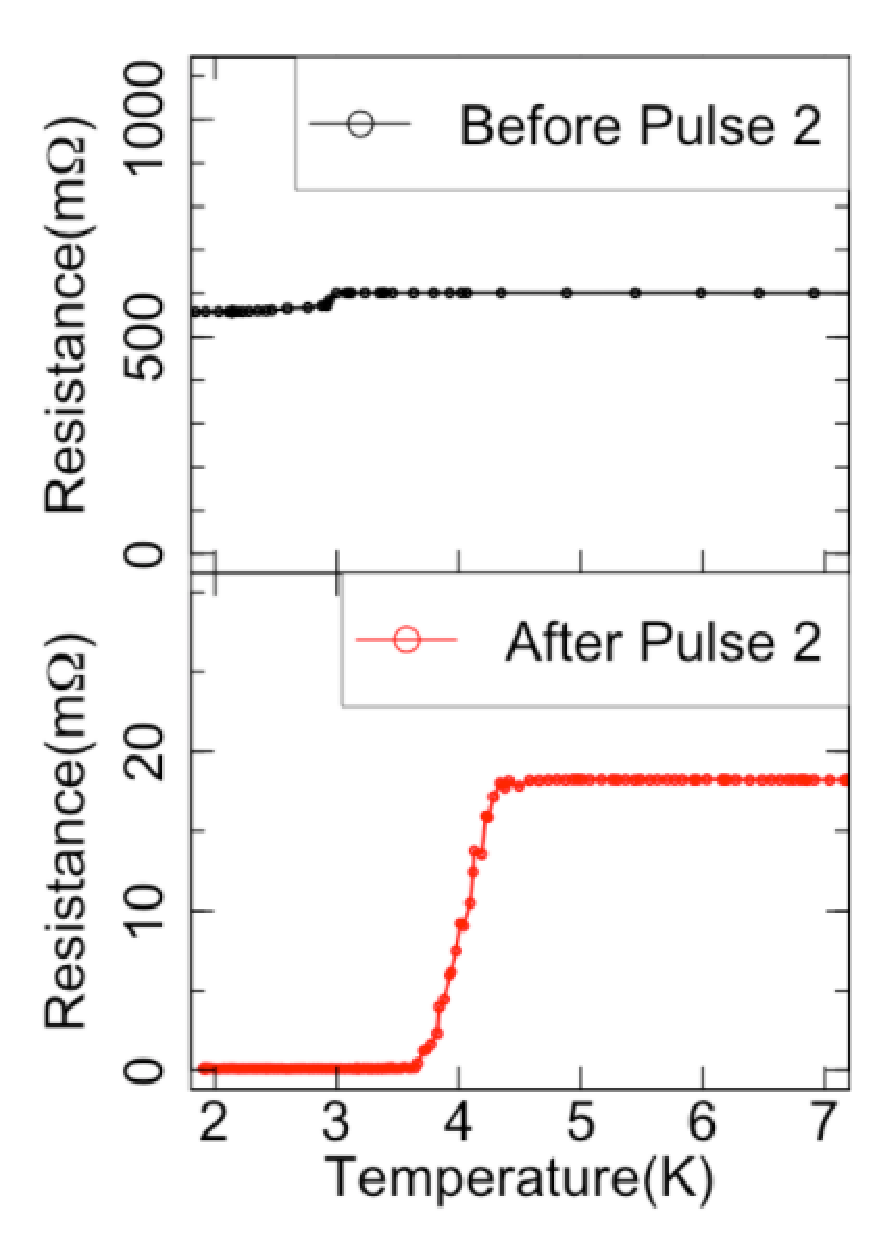
\includegraphics[width=0.4\hsize]{results_discussions/low1.eps}
  \end{center}
  \caption{試料6-1の低温での抵抗-温度依存性(2回目)}
  \label{fig:181228_after_pulse}
\end{figure}

この2回目のパルスを印加した試料6-1を3K/minで加熱してゆくと、前回の実験と同様に200Kから250Kの間で抵抗が急激に上昇した。β$\to$α転移が再び起きていることが分かる。しかし、試料の抵抗値はパルス印加する前よりも大きくなった。これは繰り返し相転移した試料に亀裂が入った結果だと筆者は考える。実際この2回目のパルスを印加した試料6-1に対して、試料に亀裂が入っていることを目視で確認した。

本実験では試料6-1に電流パルスを印加することで、半導体スズ(αスズ)から金属スズ(βスズ)への転移を実証し、金属スズが臨界温度4Kで超伝導を示すことを示した。
また同一試料に対して少なくとも2回α$\to$β変換が可能であることを示した。さらに、半導体スズ中に部分的に金属スズが共存できることを示した。
%半導体-超伝導体変換、繰り返し書き込み、部分的な書き込み

\subsection{半導体スズと金属スズの共存状態の制御}
前節では半導体スズと金属スズが共存できることを示した。しかし金属スズの体積比率はコントロールしなかった。そこで、次に半導体スズと金属スズの共存状態を電流パルスにより制御することを目指した。本節では電流パルスによりα相とβ相の共存状態を制御した実験を述べる。

25Kで行なった前節の実験に対して、本実験は室温で行なった。試料6のかけら(試料6-2)にパルス幅1秒、インターバル1秒、パルス数17のパルス列を印加し、さらにピークのパルス電流を少しずつ大きくしていった。温度上昇しないようにインターバル中の電流は50mA(電流ピーク値の1/20)とした。

パルス中・パルス前後の顕微鏡写真と抵抗を図\ref{fig:190112summary}に示す。それぞれのパルス列に対して抵抗と外見は最初の3パルス目以降変化しなかったので、図\ref{fig:190112summary}には最初の3パルスのみ示した。パルスを印加した際の抵抗は灰色の網かけ領域で強調した。顕微鏡写真は撮影した動画から切り取ってきたもので、大きく見た目が変化しない時間帯は一枚の写真で代表させた。αスズとβスズの境界も模式図で示した。撮影中の光学的なセットアップは一定に保った。撮影後、相転移が見やすくなるようにすべての写真に対して露出とコントラス、色調を一律に調整した。
\begin{landscape}
\begin{figure}[!h]
    \begin{center}
   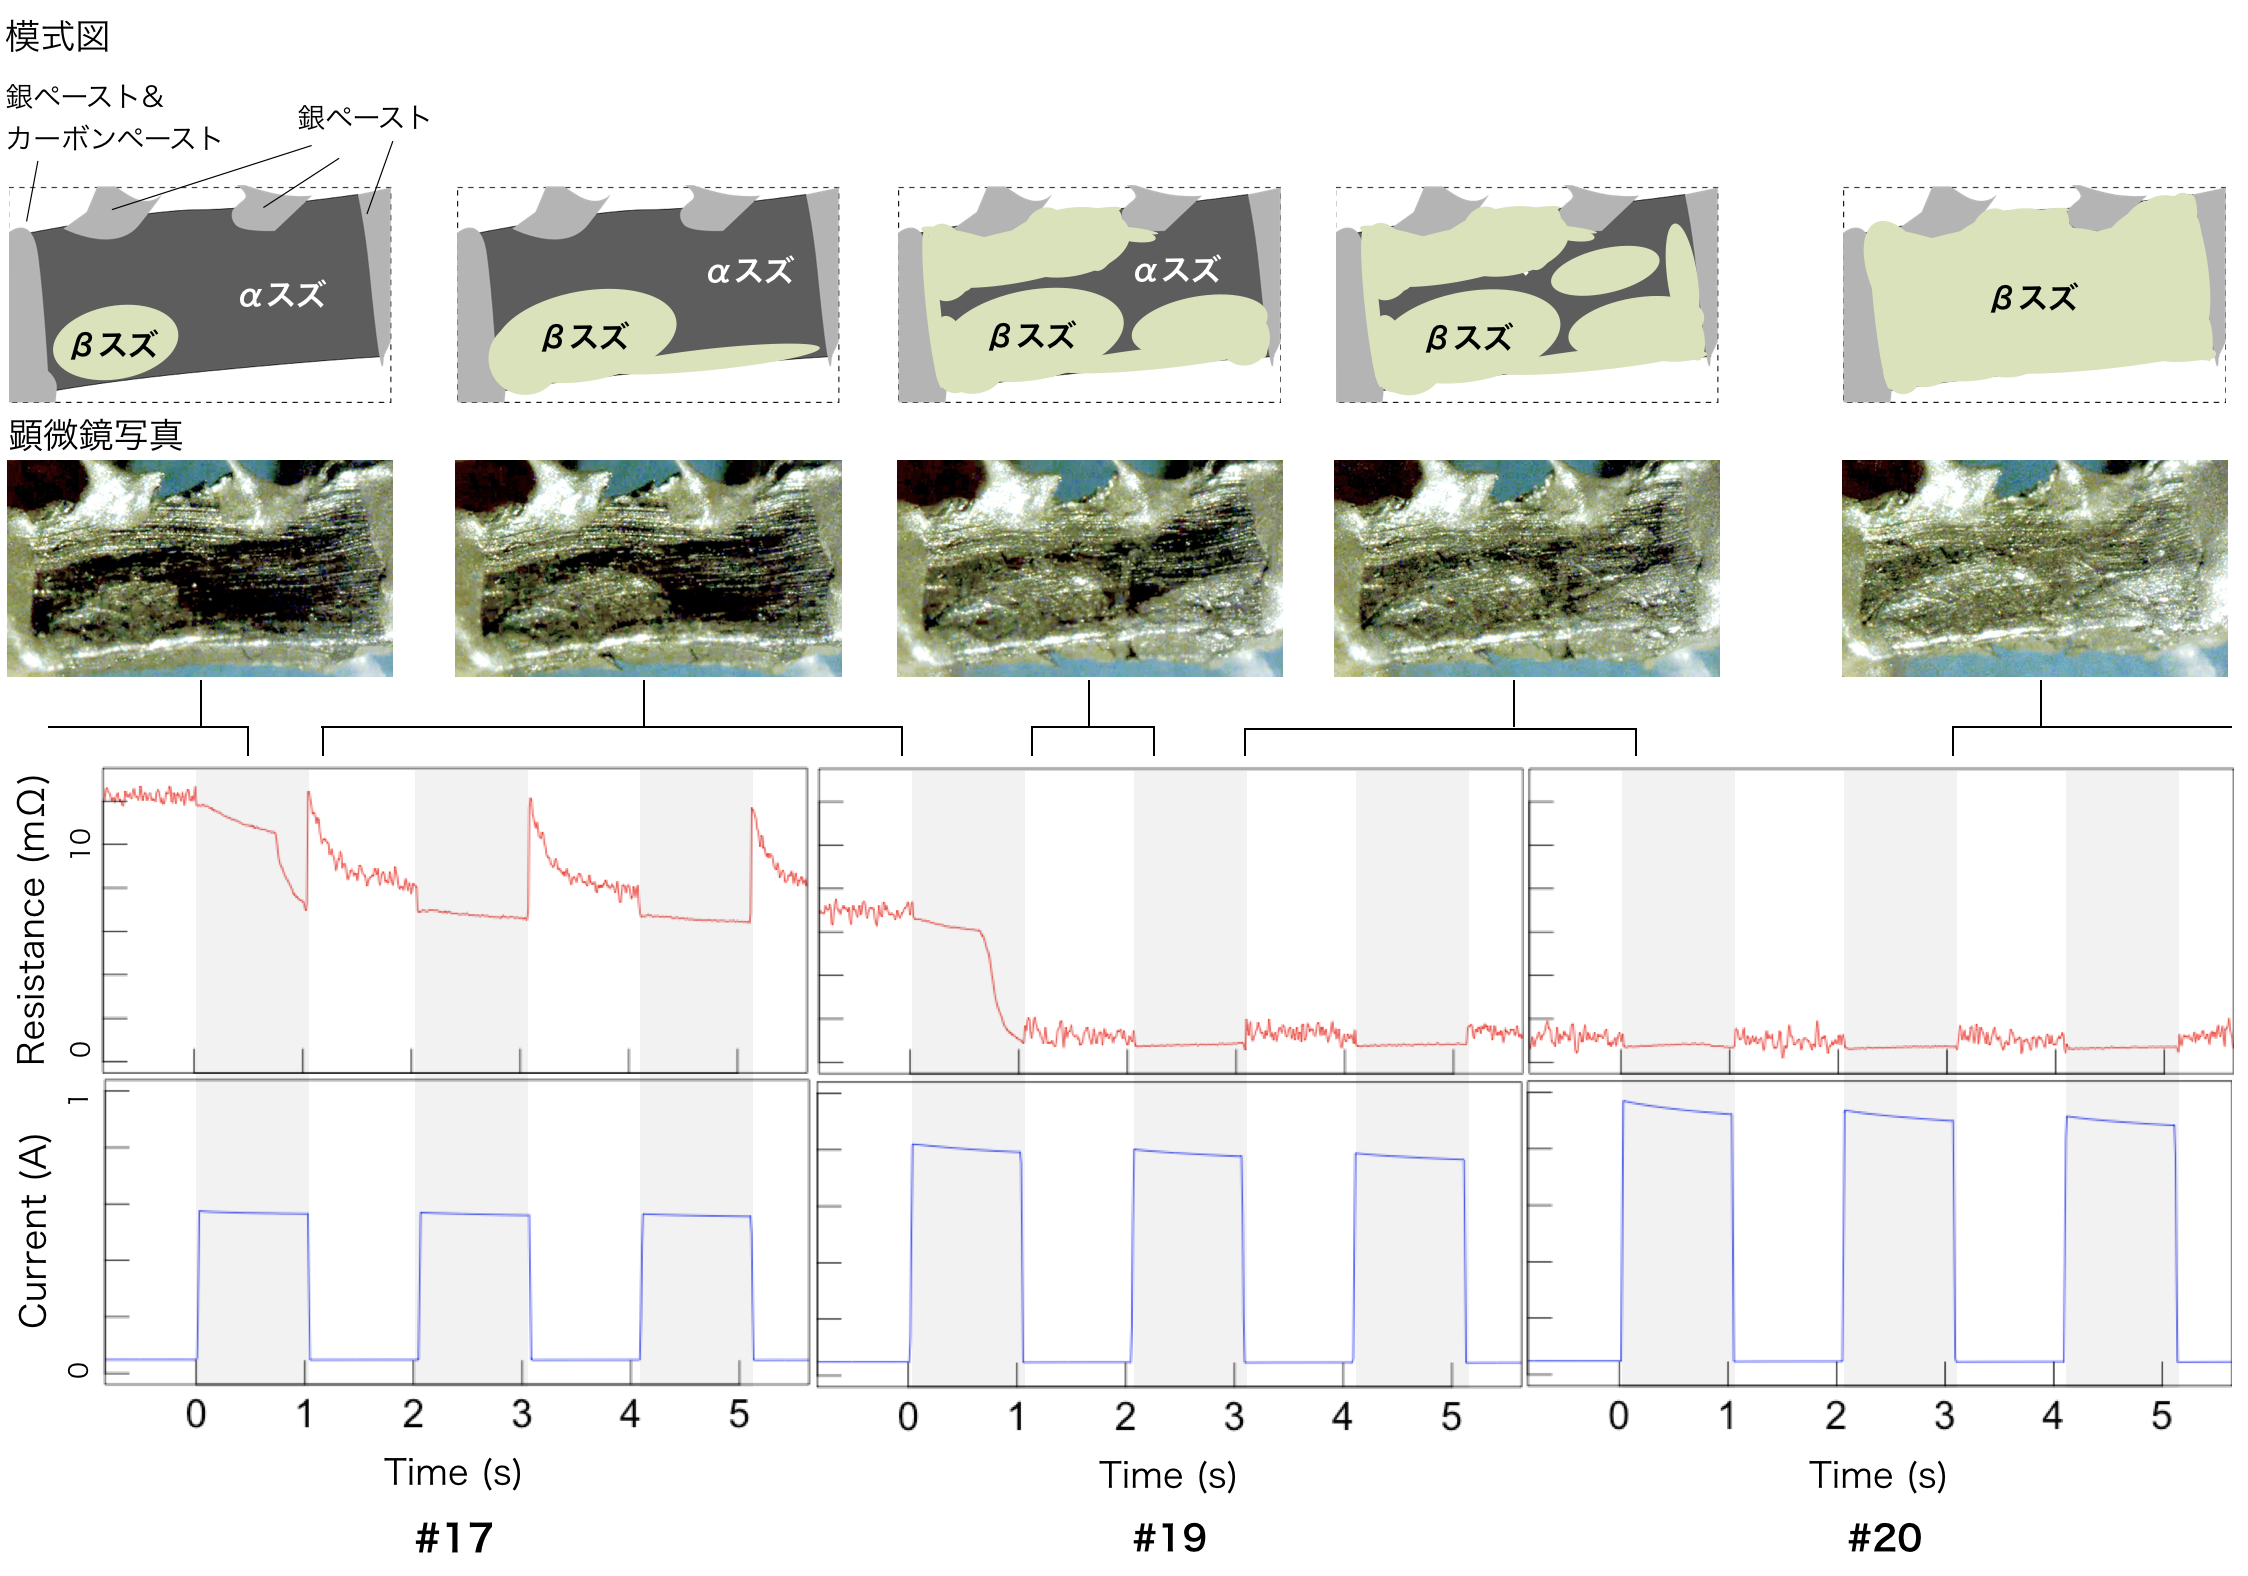
\includegraphics[width=0.9\hsize]{results_discussions/190112summary.eps}
  \end{center}
    \caption{パルス中・パルス前後の顕微鏡写真と抵抗(試料6-2)}
  \label{fig:190112summary}
\end{figure}
\end{landscape}

まず17回目のパルス列(\#17)を印加する前に得られた結果とそれに関する考察を述べる。パルス列\#16を印加する前、試料は全体的にα相だった。パルス列\#16を印加するとカーボンペーストの近く(左隅)がα$\to$β転移した。試料6のα$\to$β転移温度は350Kであるため左隅が350K程度まで温度上昇したことが分かる。しかし転移直前の全体の抵抗から温度を見積もると310Kだった。この結果は試料全体に電流パルスで数十K程度の温度勾配が付くことを示している。

17回目のパルス列を印加すると部分的にβスズを変換して、αスズとβスズが共存できることを示した。パルス列\#17を印加する前は一部に光沢のある銀色のβスズの領域が現れているが、ほとんどは黒いαスズだった。4端子法で測定した試料6-2の抵抗は11m$\Omega$程度だった。パルス\#17の1つ目のパルス(パルス\#17-1と呼ぶことにする)を印加するとα$\to$β転移が進み銀色のβスズの領域が大きくなった。顕微鏡写真を注意深く観察すると熱流出先の電圧端子(真ん中2つ)から試料の反対側で転移が進行したことが分かる。また撮影した動画から左側から右側に転移が進んでいたことも分かった。1つ目のパルスを切る直前の抵抗は6m$\Omega$(パルス列\#17を印加する前の6割程度)まで落ち込んだ。また特徴的な振る舞いとして、パルス印加直後は急激に電流が小さくなるので、インターバル中は抵抗が大きくなってから小さくなる様子が見られる。
\#17-2以降のパルスを印加しても抵抗と外見に変化は見られなかった。

19回目と20回目のパルス列を印加すると大部分をβスズに変換できた。
パルス\#19-1を印加すると、さらにα$\to$β転移が進行し銀色のβスズ
の領域が全体の半分以上を占めるようになった。この時も転移は左側から右側に向かって起きたことが分かる。抵抗は1m$\Omega$(パルス列\#17を印加する前の1/10以下)まで落ち込んだ。さらにパルス\#19-2を印加すると、抵抗に変化は見られなかったが、黒いαスズの領域はさらに小さくなりほとんどがβスズになった。抵抗に大きな変化が見られなかったことは、抵抗率の小さなβスズ(金属)がパーコレートしているとして理解できる。
パルス\#19-3以降の抵抗に変化は見られなかったが、顕微鏡写真からパルス\#20-1直後に残った黒いαスズの領域が転移しβスズとなったことが分かった。試料全体は銀色の光沢をもつようになった。

パルス列\#17の前とパルス\#20-1の後を比較すると、抵抗は1/10以下に落ち込んだ。対応するパルス列\#17を印加する前の画像(左端)とパルス列\#20を印加した後の画像(右端)を比較すると、黒色のαスズから金属的な光沢を持つβスズへの転移がはっきりと見て取れる。電流パルスによるα$\to$β変換を顕微鏡写真で可視化できた。

転移が進行する様子を詳しく見ると、相転移は熱の流入源である左側の電流端子から始まり、熱の流出先である二つの電圧端子と右側の電流端子に向かって進行していることがわかる。この振る舞いを理解するにはβスズの核が高温領域の近くで生成された可能性と、転移の進行が試料の温度勾配(数十K程度)にしたがって進行した可能性の両方を考慮する必要があると筆者は考える。筆者は本実験からどちらの要因がより支配的かについて考察できなかった。しかしいずれにせよ試料についた温度勾配を制御することが、核生成や転移の進行を制御するために有益であることと考える。

以上のカーボンペーストを用いて接続した試料に電流パルスを印加する実験の抵抗測定と光学的な観察から、α$\to$β転移の空間制御が可能であることを示した。

しかしパルス直後のインターバルで抵抗値が奇妙な振る舞いをすることも分かった。
そこで次にその特異的な振る舞いを避けるため、インターバル中の電流をすこし大きくとって80mA(ピーク値の1/10)とした実験を別の試料6のかけら(試料6-3)について行なった。パルス幅1秒、インターバル1秒、パルス数5のパルス列を印加し、ピーク電流を少しずつ大きくしながらα$\to$β転移の進行を制御した。

パルス中・パルス前後の顕微鏡写真と抵抗を図\ref{fig:190112summary}に示す。前回の実験と同様に抵抗と外見の変化は各パルス列の最初の3つのパルスでのみ起こったため、はじめの3つを示す。パルスを印加した際の抵抗は灰色の網かけ領域で強調した。顕微鏡写真は撮影した動画から切り取ってきたもので、大きく見た目が変化しない時間帯は一枚の写真で代表させた。αスズとβスズの境界も模式図で示した。撮影中の光学的なセットアップは一定に保った。撮影後、相転移が見やすくなるようにすべての写真に対して露出とコントラスト、色調を一律に調整した。
\begin{landscape}
\begin{figure}[!h]
    \begin{center}
   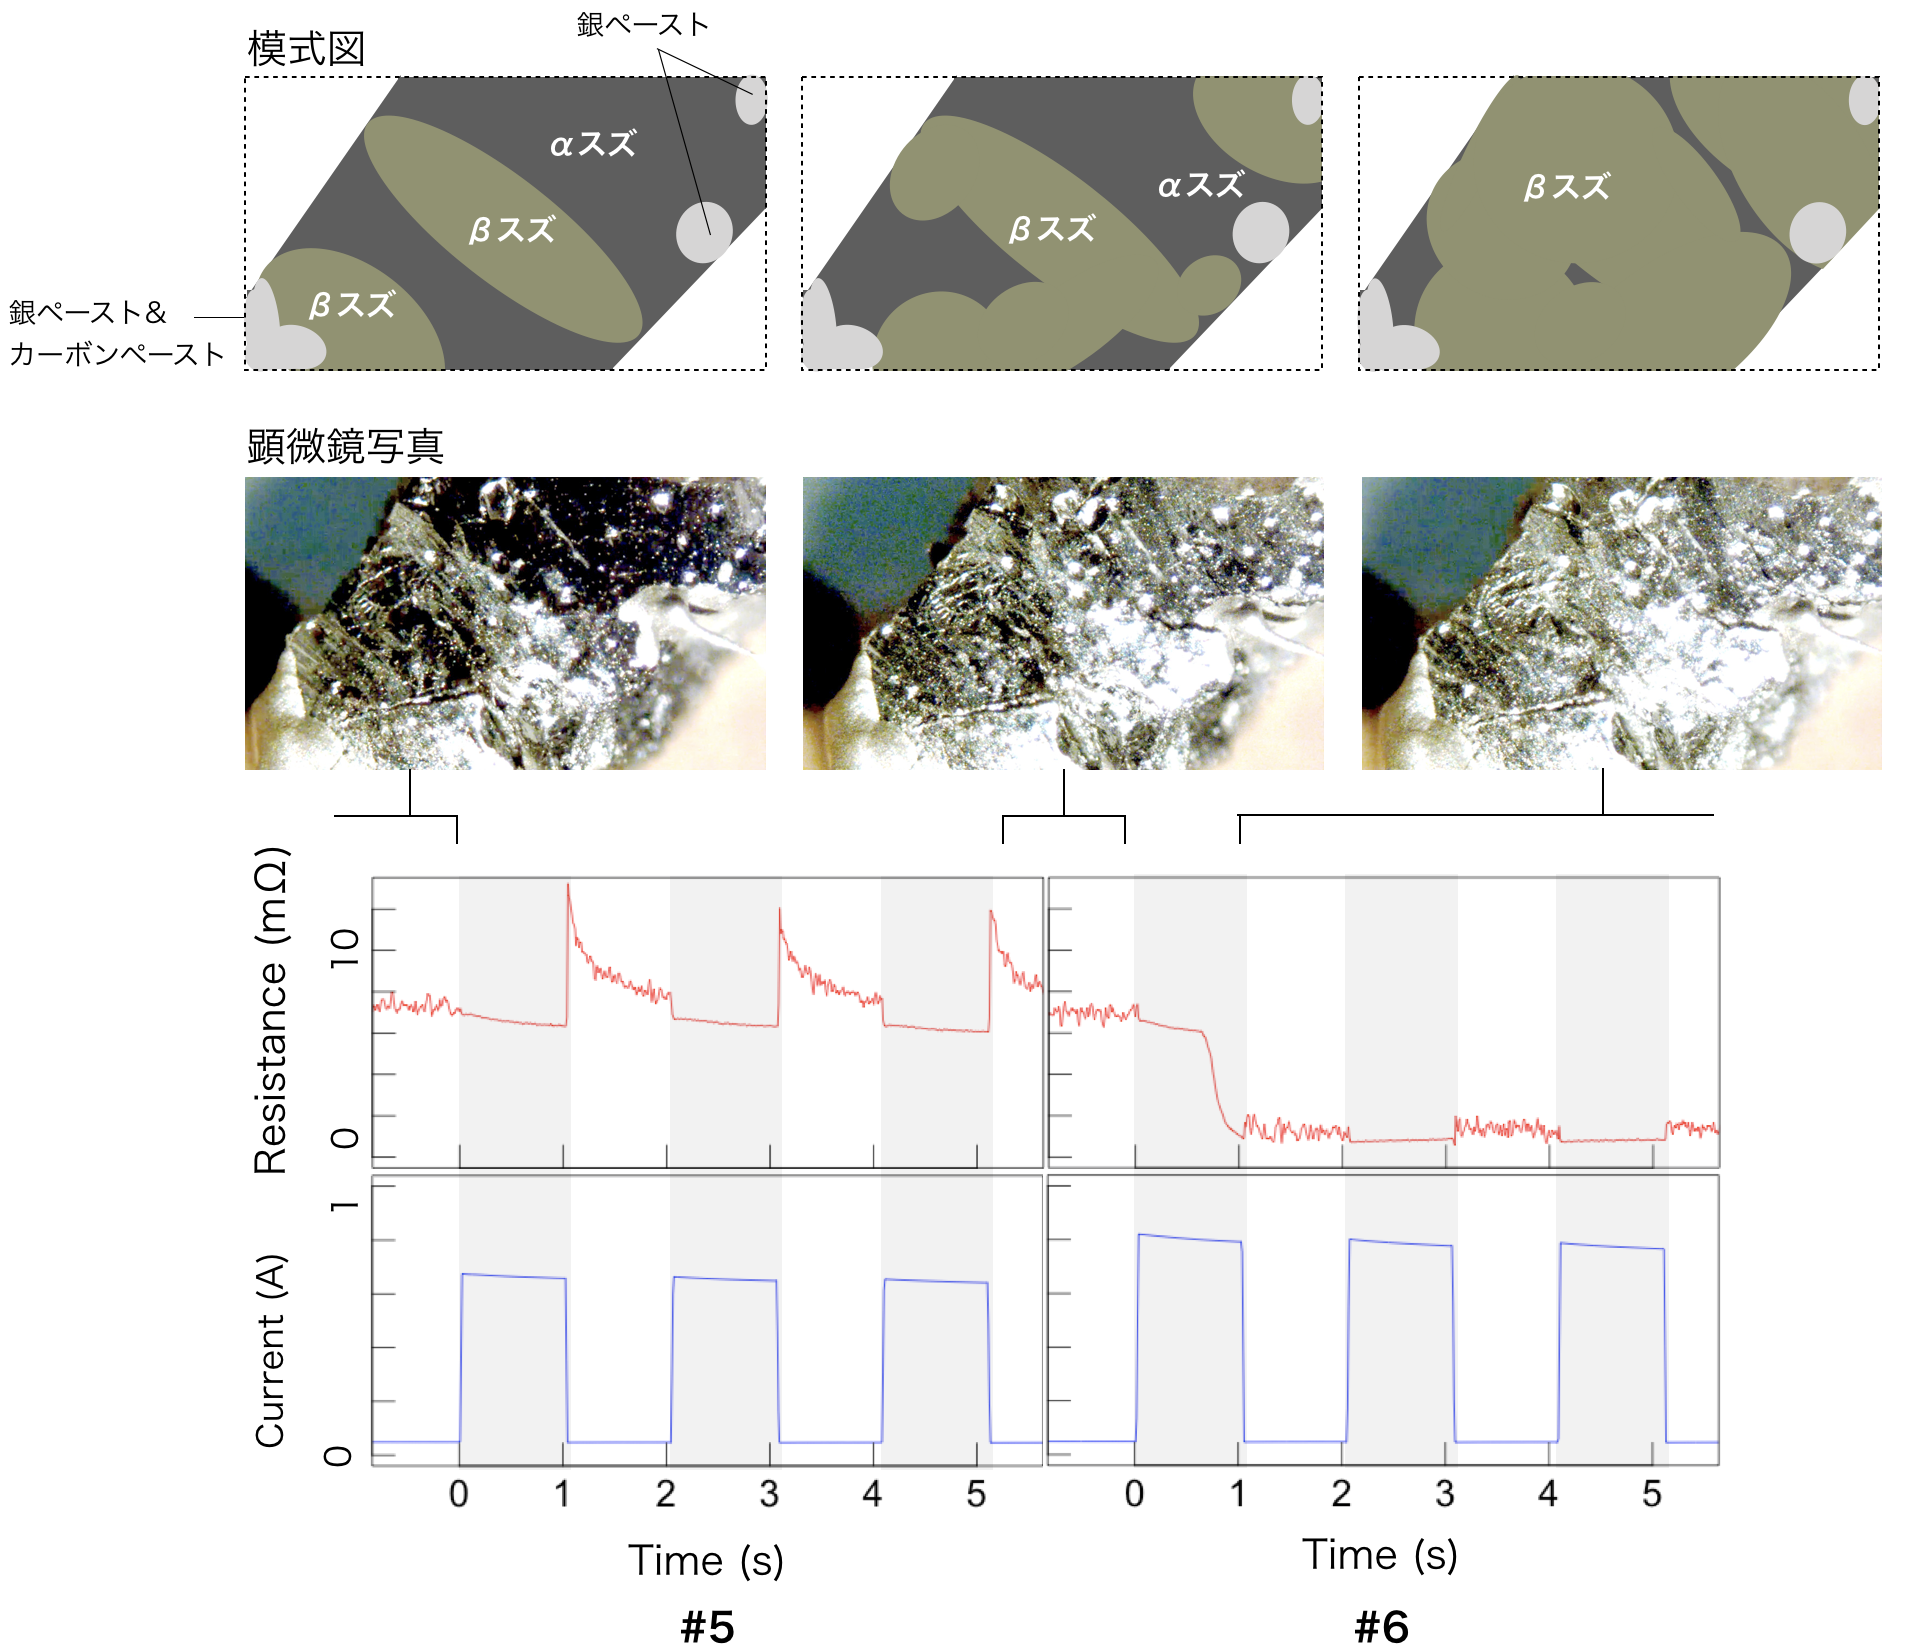
\includegraphics[width=0.75\hsize]{results_discussions/190113summary.eps}
  \end{center}
    \caption{室温におけるパルス電流印加実験の概略(試料6-3)}
  \label{fig:190113summary}
\end{figure}
\end{landscape}

パルス列\#5を印加する前は、一部(中央と下部)に光沢のある銀色のβスズの領域が現れているが多くは黒いαスズだった。4端子法で測定した試料6-2の抵抗は7m$\Omega$だった。インターバル中の電流値を大きくしたものの抵抗値は小さかった。

パルス列\#5を印加すると顕微鏡写真から光沢のあるβスズの領域が増えたことが見て取れる。パルス中の抵抗は大きく変化しなかったが、前回と同様にインターバルの抵抗が特異的な振る舞いをする。

パルス列\#6を印加すると光沢のあるβスズの領域が全体を覆うように増えたことが見て取れる。抵抗も1m$\Omega$(パルス列\#5を印加する前の1/5)以下に落ち込んだ。

本実験では光学的に金属の体積分率を評価したが、これは表面付近の情報のみを取り出したものである。また抵抗で見る情報は体積分率よりもその分布や金属の伝導経路がどのようにつながっているか(つながっていないか)に強く影響を受ける。したがって、本実験に用いた光学測定と抵抗測定では定量的な体積分率の評価は難しい。しかし定性的にはこれらは良い相関を示していると筆者は考える。

\subsection{総括}
半導体スズの試料6に対して、電流パルスによる加熱・急冷を適用すると、半導体スズは金属スズへと変化した。パルス印加直後の冷却速度は$10^2$ K/s程度であり、パルスによって生成された金属スズは3.7K以下でゼロ抵抗を示した。以上の結果は、電流パルスによる半導体から超伝導体への不揮発変換に成功したことを意味している。このように、パルス加熱・急冷を用いた生成法がIrTe$_2$以外の物質系に適用できることを実証し、大きな抵抗変化を伴う超伝導生成を実現した。

さらに、パルス印加中に相転移が進行する様子を、光学顕微鏡を用いた実空間観測によって調べた。この測定により、半導体-超伝導変換に使用する電流パルスの強度を調節することで、半導体スズと金属スズの共存状態を生成できることを示した。共存状態の実現は、光を用いた局所加熱によって、半導体スズ中に金属スズを書き込むことが可能であることを示唆している。したがって、この知見は光リソグラフィによる超伝導回路の書き込みに応用することができる。

%\subsection{電流パルスを用いたβ相からα相への変換}

\clearpage

%cd Documents/GitManagedProjects-Kagawalab/報告書/卒業論文/results_discussions/